
\documentclass[landscape,norsk,11pt]{seminar} 
 
\def\everyslide{\sf}
\usepackage{babel}
\usepackage{ucs}
\usepackage[utf8x]{inputenc}

\usepackage[T1]{fontenc}

\usepackage{hyperref}
\usepackage{graphics}

\slideframe{none}

\title{CG3 in dialogue systems - Vasta and Sahka}

\author{Lene Antonsen, Biret Ánne Bals Baal\\
Saara Huhmarniemi, Trond Trosterud \\
 \scalebox{0.30}[0.30]{
\includegraphics{img/logoWeb070sh.jpg}} \\
  \textit{http://giellatekno.uit.no/oahpa/}}
%  \scalebox{0.10}[0.10]{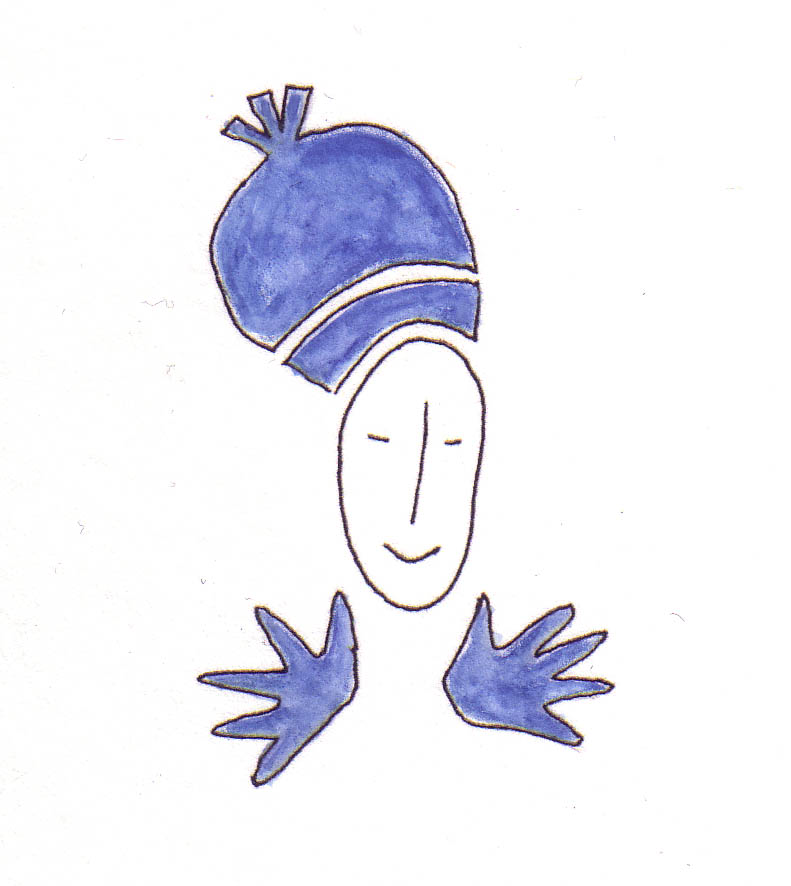
\includegraphics{img/vasta.png}} \\
\begin{document}
\begin{slide}

\maketitle

\newslide
\textbf{Pedagogical programs for learning sámi with QA}\\
\newline
\textbf{Vasta}: The program generates questions, the student can answer quite freely - with grammatical feedback \\ \newline
\textbf{Sahka}: A written dialogue between the program and the student - the answer decides the progress of the dialogue.

\newslide
\textbf{Vasta}
\scalebox{0.90}[0.90]{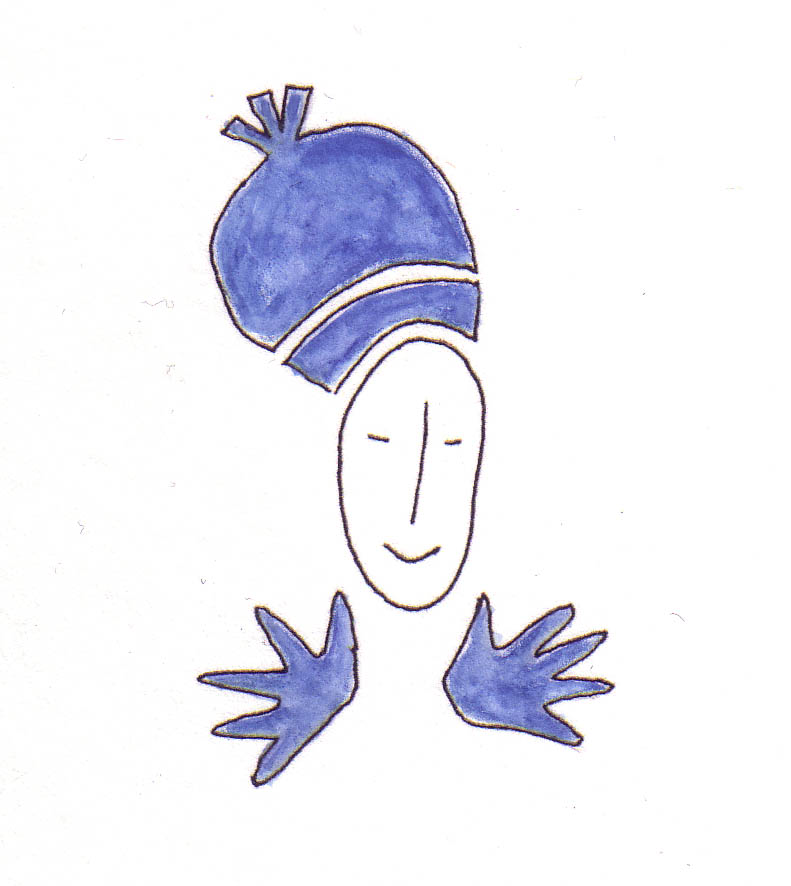
\includegraphics{img/vasta.png}} \\

\newslide
\textbf{Generating questions}
\scalebox{.35}[.35]{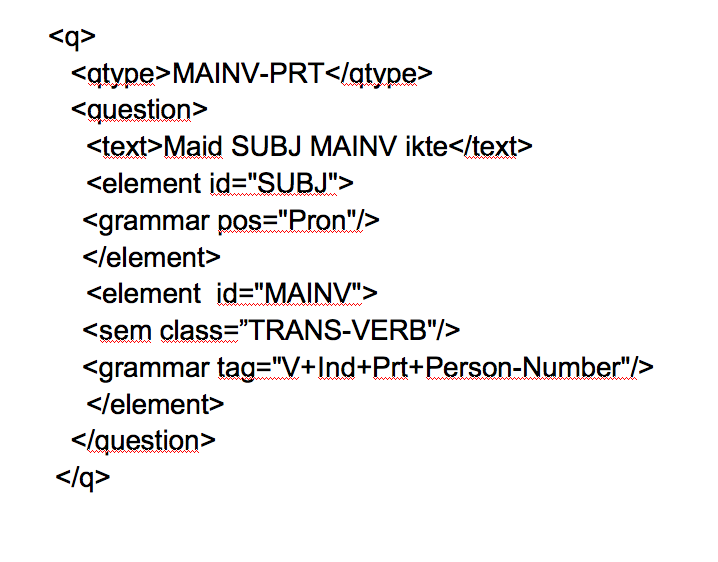
\includegraphics{img/xml_question.png}}



\newslide
\textbf{Maid don lohket ikte?}
(What did you read yesterday?) \\
Acceptable answers:
\begin{itemize}
\item Mun han lohken ollu \'aviissaid. (I read many newspapers.)
\item Ikte mun gal lohken buori girjji. (Yesterday I read a good book.)
\item In lohkan maidege. (I did not read anything.)
\item Ikte in lohkan. (Yesterday I did not read.)
\end{itemize}

\newslide
\textbf{Maid don lohket ikte?}
(What did you read yesterday?) \\
Incorrect answers:
\begin{itemize}
\item Mun lohket ollu \'aviissaid. (Not agreement subj/verbal.)
\item Mun lohken ollu áviissat. (Object should be in accusative.)
\end{itemize}


\newslide
\textbf{Steps}

\begin{enumerate}
\item Analyse (morph-disambiguate) the question and answer together
\item Common CG up until mapping. The disambiguation is incomplete, since we are careful with the errouneous input
\item Select the relevant reading
\item Make \&err assignment mapping rules
\item > message to the student
\end{enumerate}

\newslide
\textbf{Integrating the spellchecker in our ped program}

\newslide
\textbf{Didactics more important than pragmatics} \\
The goal is to train morphology -- therefore:
\begin{itemize}
\item{No elipsis							  }
\item{Finite verb compulsatory}
\item{No inclusive 1st person dual and plural}
\item{The answer \textit{I do not know} is not accepted}
\end{itemize}


\newslide
\textbf{Answer with the same verb}

Solution: Sticky tag with regex (thanks to Tino)

Exceptional handling of pro-verbs 

\newslide
\scalebox{.50}[.50]{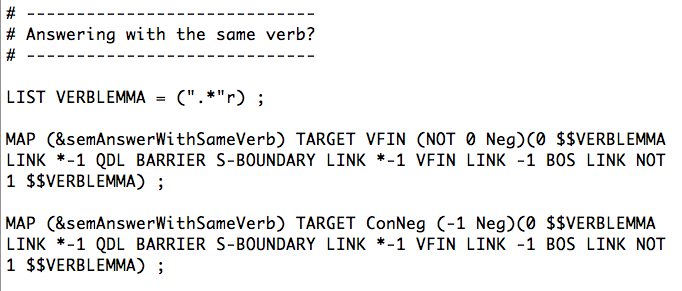
\includegraphics{img/answering_same_verb.png}}


\newslide

\textbf{The errors are ordered:}
%The student gets one error message at a time, corrects according to that, and eventually gets a new error message again.
\begin{enumerate}
\item spelling-error
\item verb: finit/infinit, what kind of verb,...
\item agreement subj/verbal
\item person/number and tense according to question
\item case of noun, according to question and argument of verb 
\item case and type of numeral
\item PP: case and type of adp
\item agreement inside NP
\item time-expression, place-expressions, some particles
\end{enumerate}


\newslide
\textbf{Unintended lemmas, lexical level} \\
How to cope with unintended lemmas?

Problem e.g. \textit{viessut} (a rare verb) \\
Possible solutions:

\begin{itemize}
\item{Remove lemmas from the analyser, and get a question mark}
\item{Make a lexeme-specific rule for the \textit{viessu / viessut} pair}
\item{Make a set of the problematic lemmas/word forms, and change the reading}
\end{itemize}


\newslide
\textbf{Marginal morphological analyses} \\
e.g. possessive suffixes \\
> Remove them (when there is another reading)

When it is the only reading, \\ e.g. Px \& strong grade vs. Loc \& weak grade: \\
> Give a comment about it to the student



%\newslide

%QA information retrieval how to process questions
%interactive, aske the user for clarification

%QA: 

%Question matrixes: generate a set of questions

\newslide
\textbf{An example -- from a test student}
%The output is manipulated  - it would not give two mappings to the same reading.
\scalebox{.32}[.35]{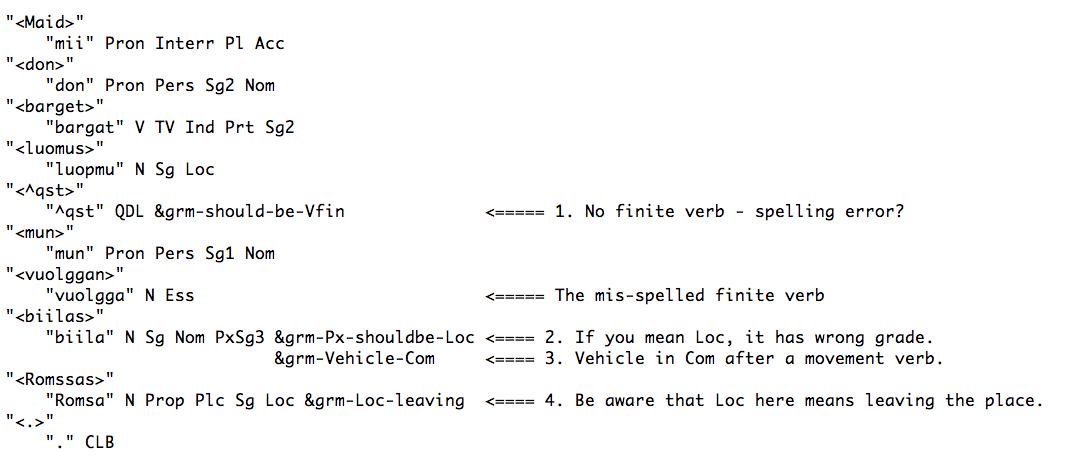
\includegraphics{img/sentence_example.png}}

\newslide
\textbf{Sahka}
\scalebox{0.90}[0.90]{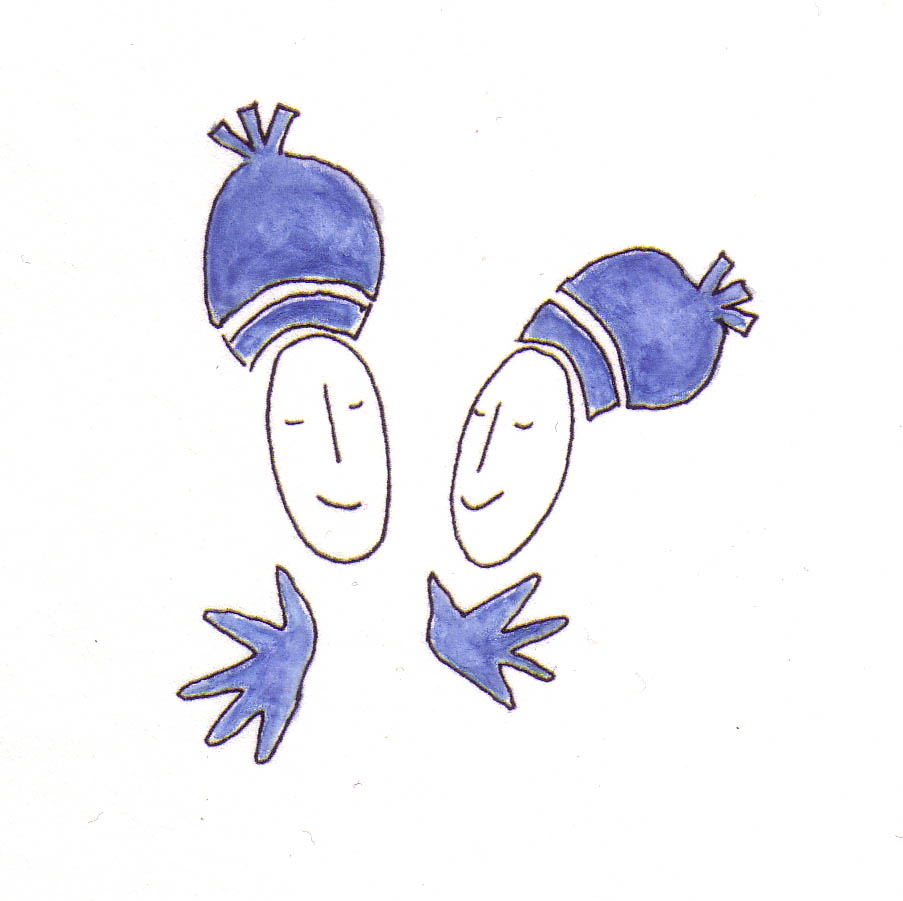
\includegraphics{img/sahka.png}} \\

\newslide
Negative or affirmative \\
One of them as default -- in case of difficulties in the analyse.

\newslide
\textbf{Negative or affirmative answer?}
\scalebox{.35}[.35]{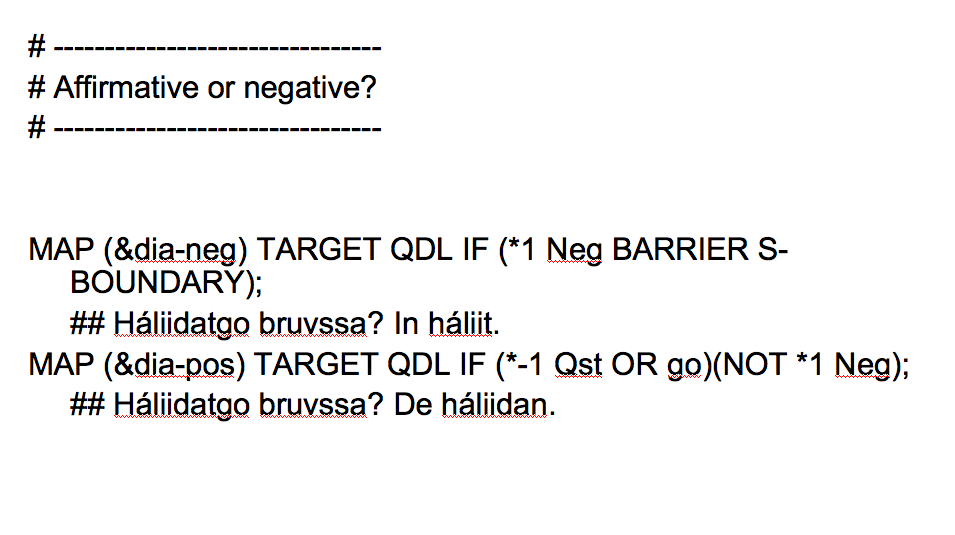
\includegraphics{img/aff_or_neg.png}}



\newslide
\textbf{Names}\\
a string or a Prop  (LIST QMRK = ? ; )
\scalebox{.30}[.30]{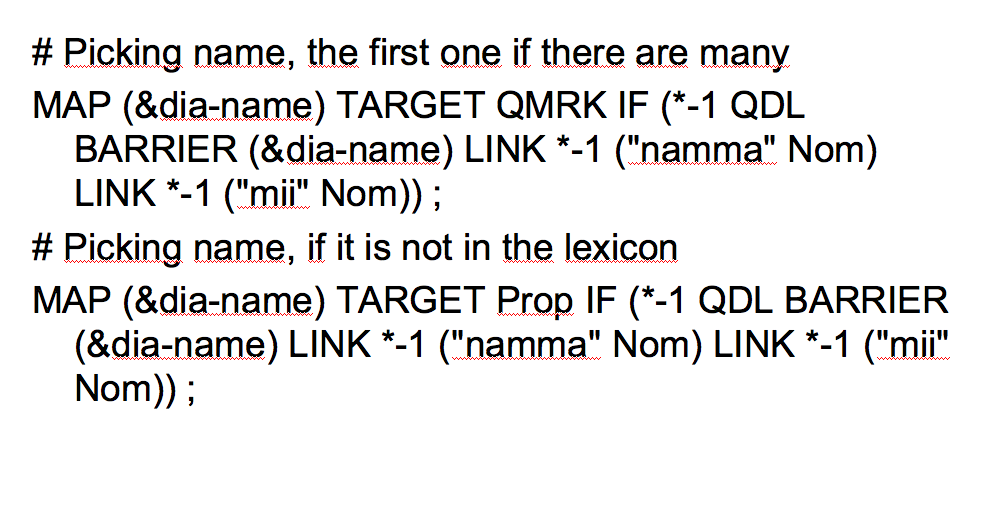
\includegraphics{img/picking_name.png}}

\newslide
\textbf{Picking the age with regex}\\
for progress of the dialogue \\

\&dia-adult \\
\&dia-young \\
\&dia-child









\end{slide}
\end{document}




